\documentclass[space,nooutcomes]{ximera} 

% For preamble materials

\usepackage{pgf,tikz}
\usepackage{mathrsfs}
\usetikzlibrary{arrows}
\usepackage{framed}
\usepackage{amsmath}
\pgfplotsset{compat=1.16}

\usepackage{numprint} % For printing large numbers with commas. 
\npthousandsep{,}


\graphicspath{
  {./}
  {quickQuestions/}
  {ximeraTutorial/}
}


\pdfOnly{\renewenvironment{image}[1][]{\begin{center}}{\end{center}}}

%%% This set of code is all of our user defined commands
\newcommand{\bysame}{\mbox{\rule{3em}{.4pt}}\,}
\newcommand{\N}{\mathbb N}
\newcommand{\C}{\mathbb C}
\newcommand{\W}{\mathbb W}
\newcommand{\Z}{\mathbb Z}
\newcommand{\Q}{\mathbb Q}
\newcommand{\R}{\mathbb R}
\newcommand{\A}{\mathbb A}
\newcommand{\D}{\mathcal D}
\newcommand{\F}{\mathcal F}
\newcommand{\ph}{\varphi}
\newcommand{\ep}{\varepsilon}
\newcommand{\aph}{\alpha}
\newcommand{\QM}{\begin{center}{\huge\textbf{?}}\end{center}}

\renewcommand{\le}{\leqslant}
\renewcommand{\ge}{\geqslant}
\renewcommand{\a}{\wedge}
\renewcommand{\v}{\vee}
\renewcommand{\l}{\ell}
\newcommand{\mat}{\mathsf}
\renewcommand{\vec}{\mathbf}
\renewcommand{\subset}{\subseteq}
\renewcommand{\supset}{\supseteq}
\renewcommand{\emptyset}{\varnothing}
\newcommand{\xto}{\xrightarrow}
\renewcommand{\qedsymbol}{$\blacksquare$}
\newcommand{\bibname}{References and Further Reading}
\renewcommand{\bar}{\protect\overline}
\renewcommand{\hat}{\protect\widehat}
\renewcommand{\tilde}{\widetilde}
\newcommand{\tri}{\triangle}
\newcommand{\minipad}{\vspace{1ex}}
\newcommand{\leftexp}[2]{{\vphantom{#2}}^{#1}{#2}}

%% More user defined commands
\renewcommand{\epsilon}{\varepsilon}
%\renewcommand{\theta}{\vartheta} %% only for kmath
\renewcommand{\l}{\ell}
\renewcommand{\d}{\, d}
\newcommand{\ddx}{\frac{d}{dx}}
\newcommand{\dydx}{\frac{dy}{dx}}


\usepackage{bigstrut}


\newenvironment{sectionOutcomes}{}{}

\usepackage{array}
%\setlength{\extrarowheight}{-.2cm}   % Commented out by Findell to fix table headings.  Was this for typesetting division?  
\newdimen\digitwidth
\settowidth\digitwidth{9}
\def~{\hspace{\digitwidth}}
\def\divrule#1#2{
\noalign{\moveright#1\digitwidth
\vbox{\hrule width#2\digitwidth}}}


\title{Integer Arithmetic}
\author{Brad Findell}
\begin{document}
\begin{abstract}
Exploring arithmetic of integers.  
\end{abstract}
\maketitle


To explain integer arithmetic, here are some ideas: 
\begin{enumerate}
\item Patterns
\item Fact families
\item Algebraic reasoning
\item Models, red and black chips, walking on a number line, checks and bills, etc. 
\end{enumerate}


\section*{Integers as Directed Segments}

Integers $4$ and $-3$ as points: 

  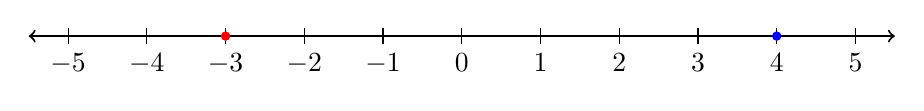
\begin{tikzpicture}
    \draw[<->, line width=.75pt] (-5.5,0) -- (5.5,0);
    \foreach \i in {-5,-4,...,5} % numbers on line
      \draw (\i,0.1) -- + (0,-0.2) node[below] {\normalsize $\i$}; % tick and their labels
	\fill[red] (-3,0) circle (0.6 mm);
	\fill[blue] (4,0) circle (0.6 mm);
  \end{tikzpicture}
  
Integers $4$ and $-3$ as vectors: 

    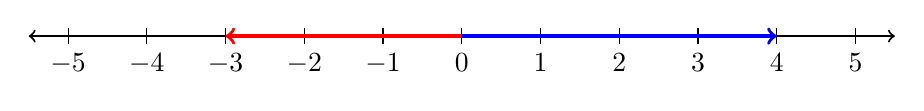
\begin{tikzpicture}
    \draw[<->, line width=.75pt] (-5.5,0) -- (5.5,0);
    \foreach \i in {-5,-4,...,5} % numbers on line
      \draw (\i,0.1) -- + (0,-0.2) node[below] {\normalsize $\i$}; % tick and their labels
	\draw[red, ->, line width=1.25pt] (0,0) -- (-3,0);
	\draw[blue, ->, line width=1.25pt] (0,0) -- (4,0);
   \end{tikzpicture}
   
Integer sum, $4 + -3$ as point + vector:  

    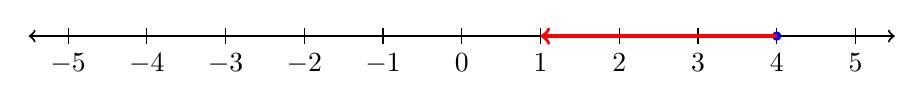
\begin{tikzpicture}
    \draw[<->, line width=.75pt] (-5.5,0) -- (5.5,0);
    \foreach \i in {-5,-4,...,5} % numbers on line
      \draw (\i,0.1) -- + (0,-0.2) node[below] {\normalsize $\i$}; % tick and their labels
	\fill[blue] (4,0) circle (0.6 mm);
	\draw[red, ->, line width=1.25pt] (4,0) -- (1,0);
   \end{tikzpicture}

Integer sum, $4 + -3$ as vector + vector:  

    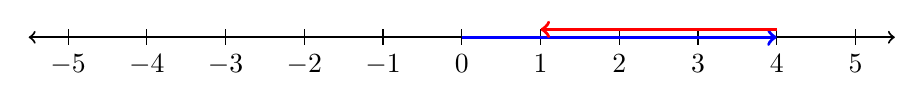
\begin{tikzpicture}
    \draw[<->, line width=.75pt] (-5.5,0) -- (5.5,0);
    \foreach \i in {-5,-4,...,5} % numbers on line
      \draw (\i,0.1) -- + (0,-0.2) node[below] {\normalsize $\i$}; % tick and their labels
	\draw[blue, ->, line width=1.25pt] (0,0) -- (4,0);
 	\draw[red, ->, line width=1.25pt] (4,0.1) -- (1,0.1);
   \end{tikzpicture}

\dots and we can think of the sum as a point or as a vector.  




\end{document}
